\documentclass{beamer}
\usetheme{Boadilla}
\usepackage{tikz}
\usepackage{graphicx}
\usepackage{amsmath}
\usetikzlibrary{shapes.geometric,arrows, positioning, fit}




\title{Weekly Presentation}
\subtitle{Week 46}
\author{}
\institute{Luleå University of Technology}
\date{\today}



\begin{document}
\begin{frame}
    \titlepage
\end{frame}

\begin{frame}
    \frametitle{Overview}
    \tableofcontents
\end{frame}

%%%%%%%%%%%% Add new frames below this line %%%%%%%%%
\section{Status update}
\subsection{Milestone review}
\begin{frame}
    \frametitle{Milestones}
    \centering
    \Huge Git
\end{frame}
\subsection{Timeplan}
\begin{frame}
    \subsection{Time plan}
    \frametitle{Overall timetable}
    \begin{table}
        \begin{tabular}{| l | c | c | c | c }
            
            Sep & Oct & Nov & Dec \\
            \hline \hline
            Concept generation & Evaluation & Evaluation &  \\ 
            \hline
            Theory & Prototyping & Evaluation & Finishing up \\
            \hline
            Simulation & Evaluation & Evaluation & \\
            \hline
            Prototyping & Final Design & Evaluation &  \\
            \hline
 
        \end{tabular}
    \end{table}    
\end{frame}


\begin{frame}
    \frametitle{Time plan for September}
    \begin{table}
        \begin{tabular}{l | c | c | c | c }
        Subproject & Week 1 & Week 2 & Week 3 & Week 4 \\
        \hline \hline
            Arrowhead & Reading& Setup & API & Prototyping\\
            Movable base & Reading& Modeling & Simulation & Implementation\\
            Arm and grip  & Reading & Kinematics & Simulation& Prototyping\\
            Object detection & Reading & Testing & Prototyping & Evaluation\\
        \end{tabular}
    \end{table}
\end{frame}

\begin{frame}
    \centering
    \Huge Design
\end{frame}

\section{Design}
\subsection{Old design}
\begin{frame}
    \frametitle{Old design}
    \begin{columns}
        \begin{column}[]{0.5\textwidth}
            \begin{figure}
                \centering
                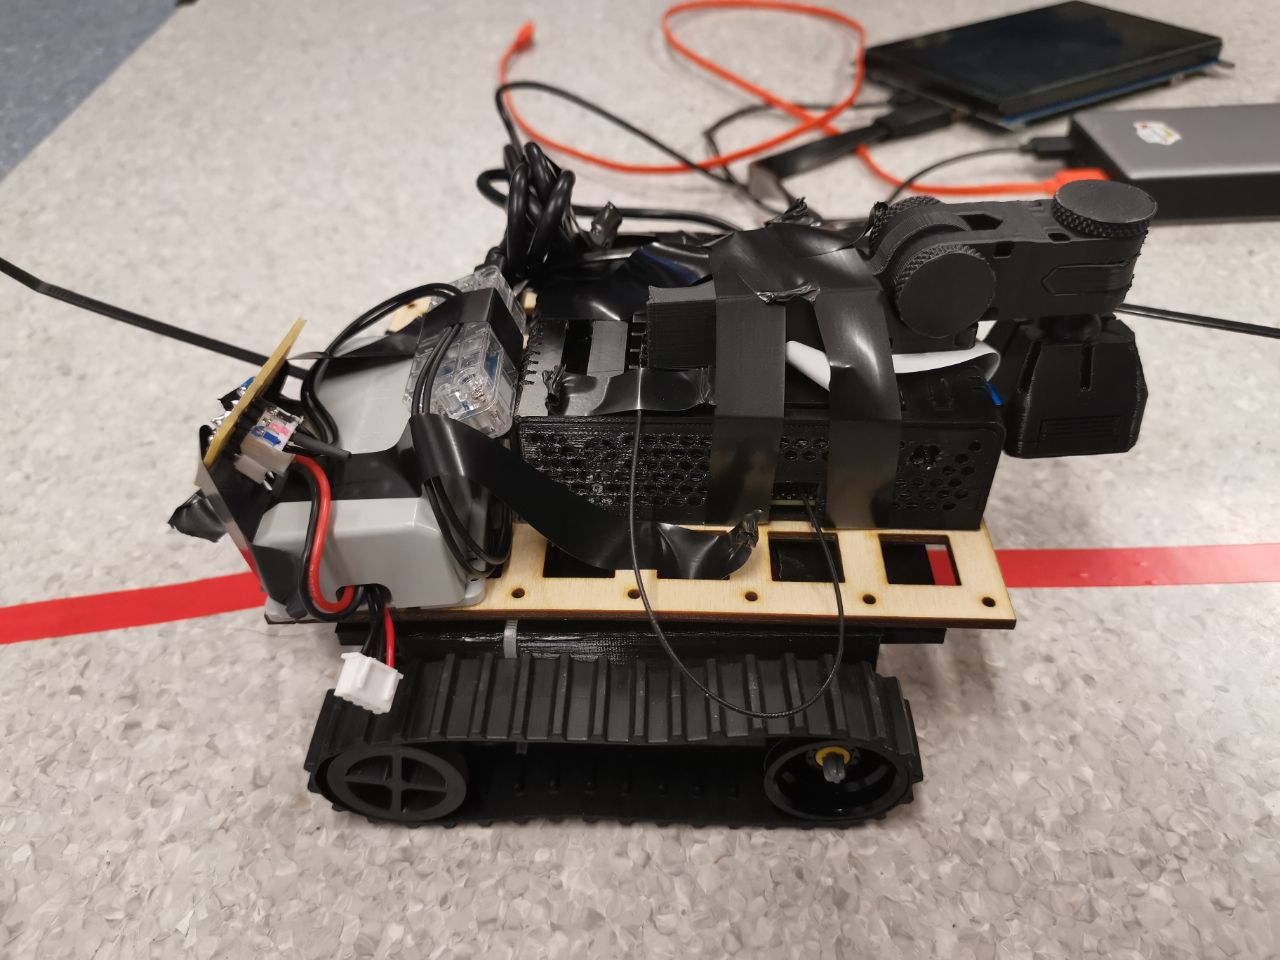
\includegraphics[width=\textwidth]{frames/img/cables.jpg}
            \end{figure}
            
        \end{column}
        \begin{column}[]{0.5\textwidth}
            \begin{figure}
                \centering
                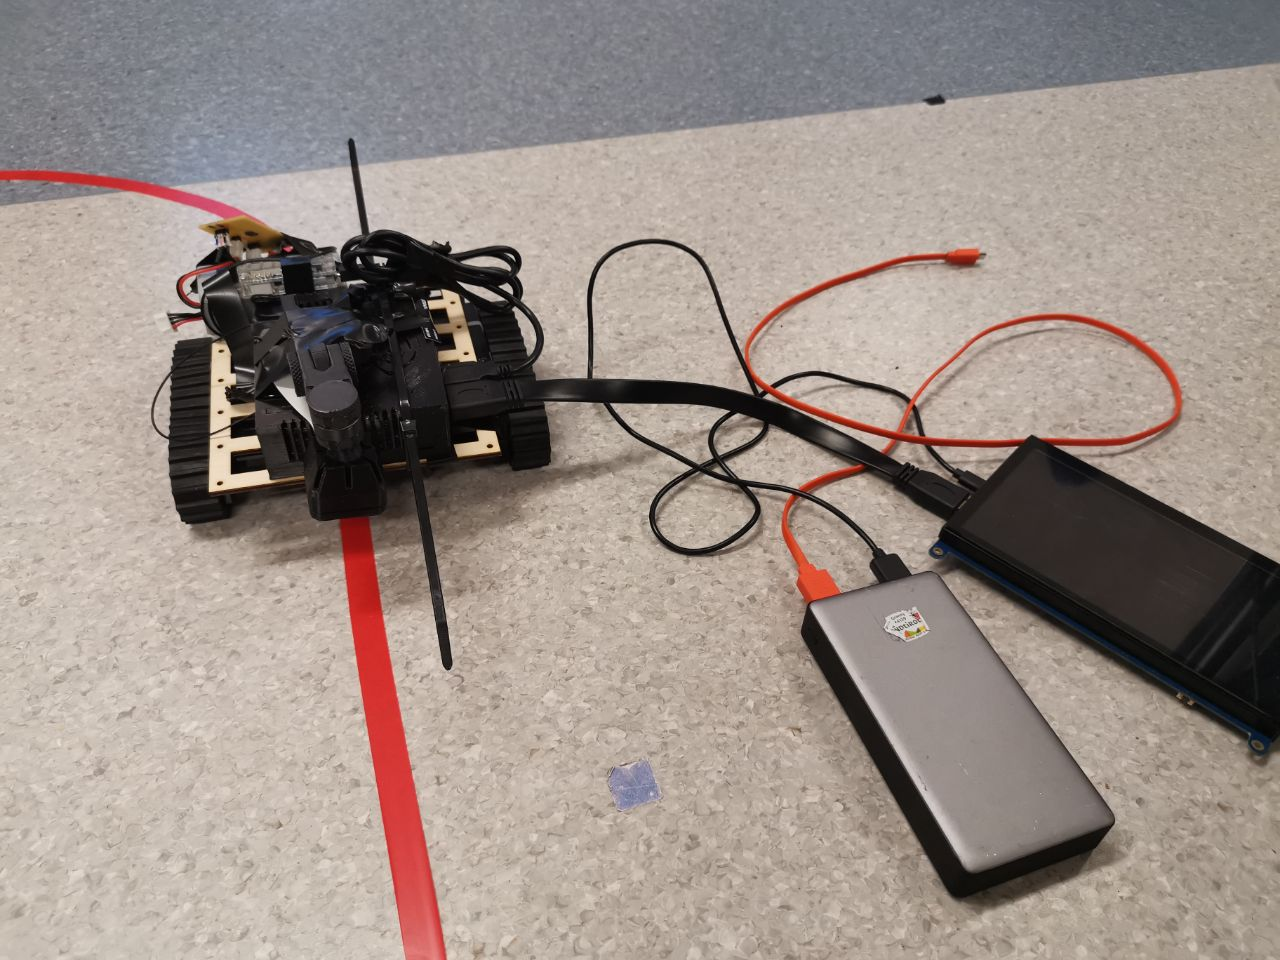
\includegraphics[width=\textwidth]{frames/img/robot.jpg}
            \end{figure}
        \end{column}
    \end{columns}
\end{frame}

\subsection{Line following}
\begin{frame}
    \frametitle{Line following}
    \begin{center}
        \Huge Video
    \end{center}
\end{frame}

\subsection{New design}
\begin{frame}
    \frametitle{New design}
    \begin{columns}
        \begin{column}[]{0.5\textwidth}
            \begin{figure}
                \centering
                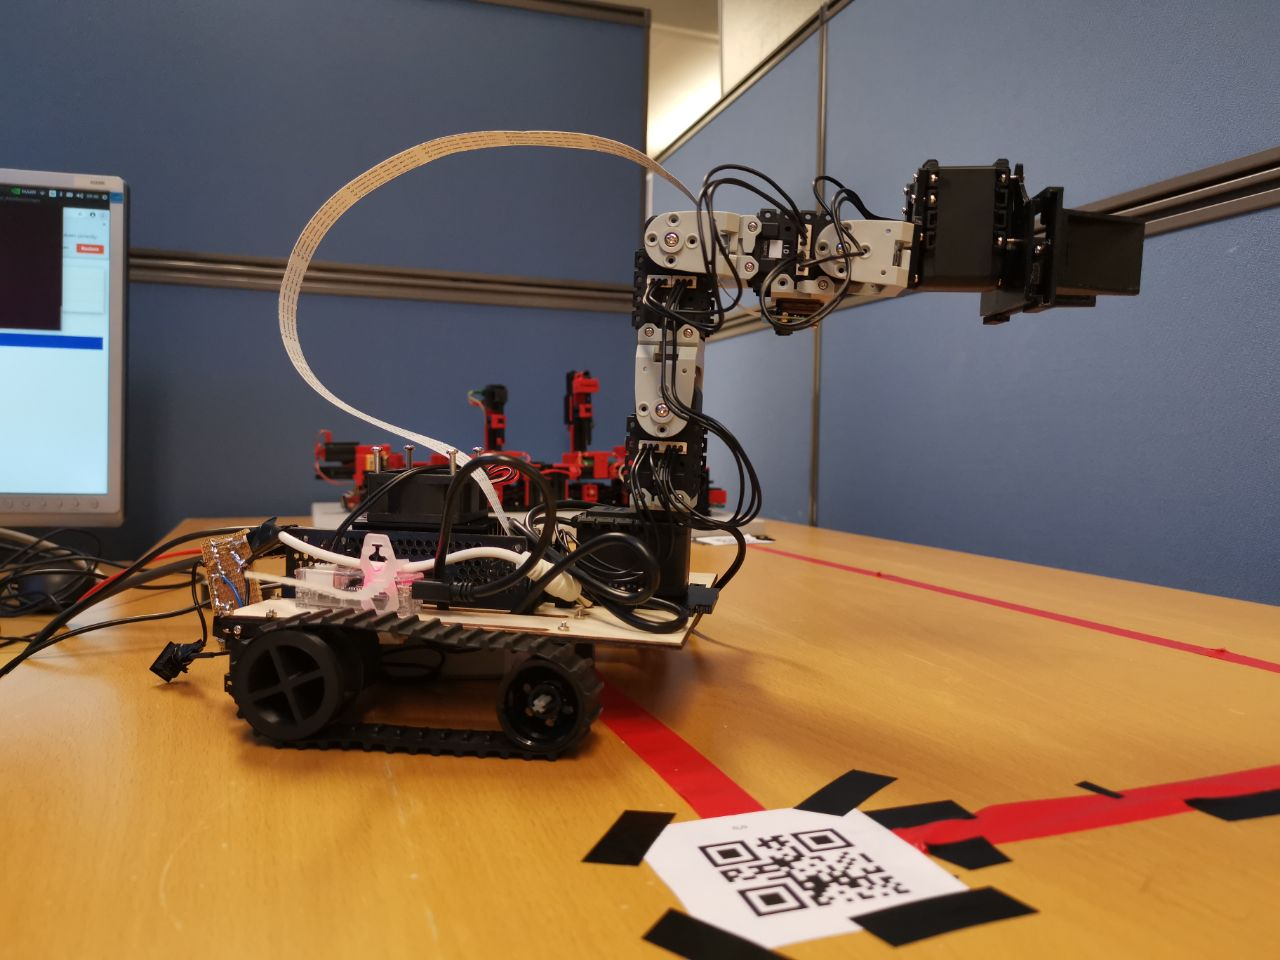
\includegraphics[width=\textwidth]{frames/img/view1.jpg}
            \end{figure}
            
        \end{column}
        \begin{column}[]{0.5\textwidth}
            \begin{figure}
                \centering
                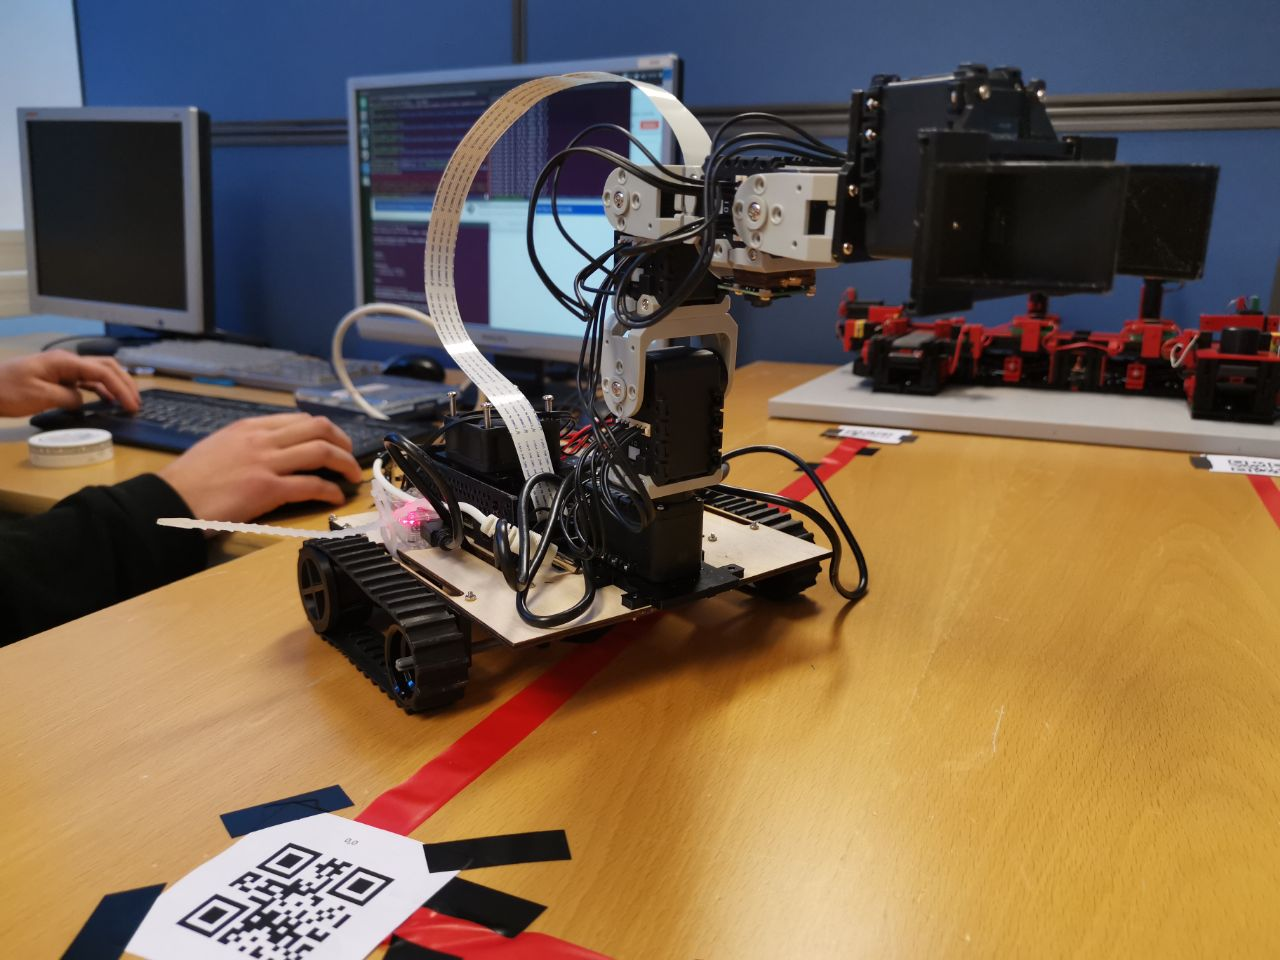
\includegraphics[width=\textwidth]{frames/img/view2.jpg}
            \end{figure}
        \end{column}
    \end{columns}
\end{frame}

\begin{frame}
    \centering
    \Huge Video
\end{frame}

\section{ToDo}
\begin{frame}
    \frametitle{ToDo}
    \begin{itemize}
        \item QR-code orientation
        \item Fusing with Arrowhead
        \item Complete the challenge
        \item Report
        \item Video
    \end{itemize}
\end{frame}




%%%%%%%%%%%% Add new frames above this line %%%%%%%%%


\begin{frame}
    \begin{center}
        \Huge Questions?
    \end{center}
\end{frame}





\end{document}